\section{Equilibrated MD}

Geometric analyses were performed to characterize the net molecular orientation of \wat~and \suldiox~molecules at different depths from the water surface. At each distance from the surface location, an orientation profile was created for both the \wat~and \suldiox~molecules. The orientation distribution for the angles $\theta$ and $\phi$ at all depths were combined to form 2D intensity plots that show how the molecular orientation distributions changed with distance to the surface location. These plots allow for a visual interpretation of how the net orientations are affected when moving from the gas phase to the surface, and then further into the aqueous bulk.

\subsection{\wat~Orientation}

The orientation depth-profiles for \wat~are shown in figure \ref{fig:water-orientation} for both the neat-water (top) and saturated (bottom) systems during the equilibrium MD simulations. In both systems the strongest orientational preference is found at the slab surfaces where the water is furthest towards the gas phase. The histograms are arranged with the plots of $\cos(\theta)$ on the left and $\cos(\phi)$ on the right columns. The surface is located at 0\angs. The angle distributions from both simulated slab surfaces were averaged for all the orientation analyses.

The bisector tilt, $\cos(\theta)$, concentrates around $\cos(\theta)=0$ within the first few\angs~of the surface, and then the distribution becomes isotropic further into the water bulk. As the tilt nears $\cos(\theta)=0$ the \wat~bisector lies within the plane of the surface indicating a water orientation either flat on the surface, or with some amount of ``twist'' sending the OH bonds in towards, or out of the bulk. The value of $\phi$ determines the ``twist'' in this case. Both systems show a peak in the distributions around $\cos(\phi)=1$ at the water surfaces. This results from an orientation of the water's y-axis (normal to the molecular plane) aligned perpendicular to the plane of the water surface. Thus, both the neat-water and saturated systems have waters lying mostly flat to the plane of the interface at a distance of 0\angs.

Although the plots show overall similarities for both the neat-water and saturated systems, the presence of a layer of adsorbed \suldiox~molecules alters the water orientation of the waters furthest into the gas phase. The waters located above 0\angs~are further into the gas phase, and interact with the layer of adsorbed \suldiox~molecules. The \suldiox~layer does not provide the same amount of strong hydrogen bonding and solvation that the waters experience further in the aqueous phase. The resulting orientation of waters above 0\angs, shown in the saturated plot of $\cos(\theta)$ of figure \ref{fig:water-orientation}, is with a bisector pointing further into the adsorbed \suldiox~gas layer, and both hydrogens pointing outward from the aqueous bulk. The effect is more pronounced further from the water phase, and above 5\angs~the $\cos(\theta)$ distribution is completely centered around $\cos(\theta)=+1$ (see figure \ref{fig:water-angles}).

%The histograms show overall similarities for both systems in their shapes and intensities from approx. 0\angs~and below. The presence of a saturated layer of adsorbed \suldiox~molecules, however, alters the water orientation, but not necessarily the orientational depth of the interface. In both $\theta$ distributions, the orientations of waters in the bulk region are isotropic until 5\angs~below the surface location. At 5\angs~below the surface the water molecules begin to orient with their bisectors within the plane of the interface (perpendicular to the surface normal, $\cos(\theta)\approx 0$). The corresponding location in the plot of $\phi$ shows that those molecules are also mostly flat to the surface ($\cos(\phi)\approx 1$). Moving further out from the bulk and into the gas phase, the distributions show $\cos(\theta)$ increasing. Waters further out from the bulk have fewer bonding interactions, and orient with their hydrogens more towards the gas phase. The bisector pointing further into the gas phase leads to isotropy in the values of $\phi$.  

The change in $\cos(\theta)$ is not as rapid at the neat-water surface as in the saturated system. Furthermore, the noise in the distribution above 5\angs~in the neat-water system is a result of fewer waters venturing beyond those extents and thus less data far from the surface. This is one indication that waters near a layer of adsorbed \suldiox~venture further above the interface and interact with the adsorbed gas molecules. The interactions with neighboring \suldiox~molecules allow the waters above the surface to orient more perpendicular to the interface. Our experimental SFG studies also predicted this reorienting behavior due to the \suldiox~interactions with the topmost surface waters.\cite{Ota2011}

The distribution of $\cos(\phi)$ is more sharply defined (i.e. less isotropic) for the neat-water system than for the saturated one. Waters on the neat surface lie flatter, whereas the presence of the \suldiox~allows a greater range of ``twist'' for those waters in the plane of the interface. The $\phi$ distributions quickly become isotropic above the surface as the bisectors orient more perpendicularly, and below the surface as the bulk water loses any orientational preference.

%Peaks in the distributions of the neat-\wat~system are more clearly pronounced as their intensities are more concentrated and larger than the surrounding area of the profiles. This difference indicates that the transition from the preferred orientation at the water surface has a sharper distinction from the isotropic bulk than in the system with the saturated \suldiox~surface. It appears that the same orientation trend is present in both systems, but the presence of the \suldiox~at the water surface decreases the degree of water orientation at the interface.

\begin{figure}[h!]
	\begin{center}
		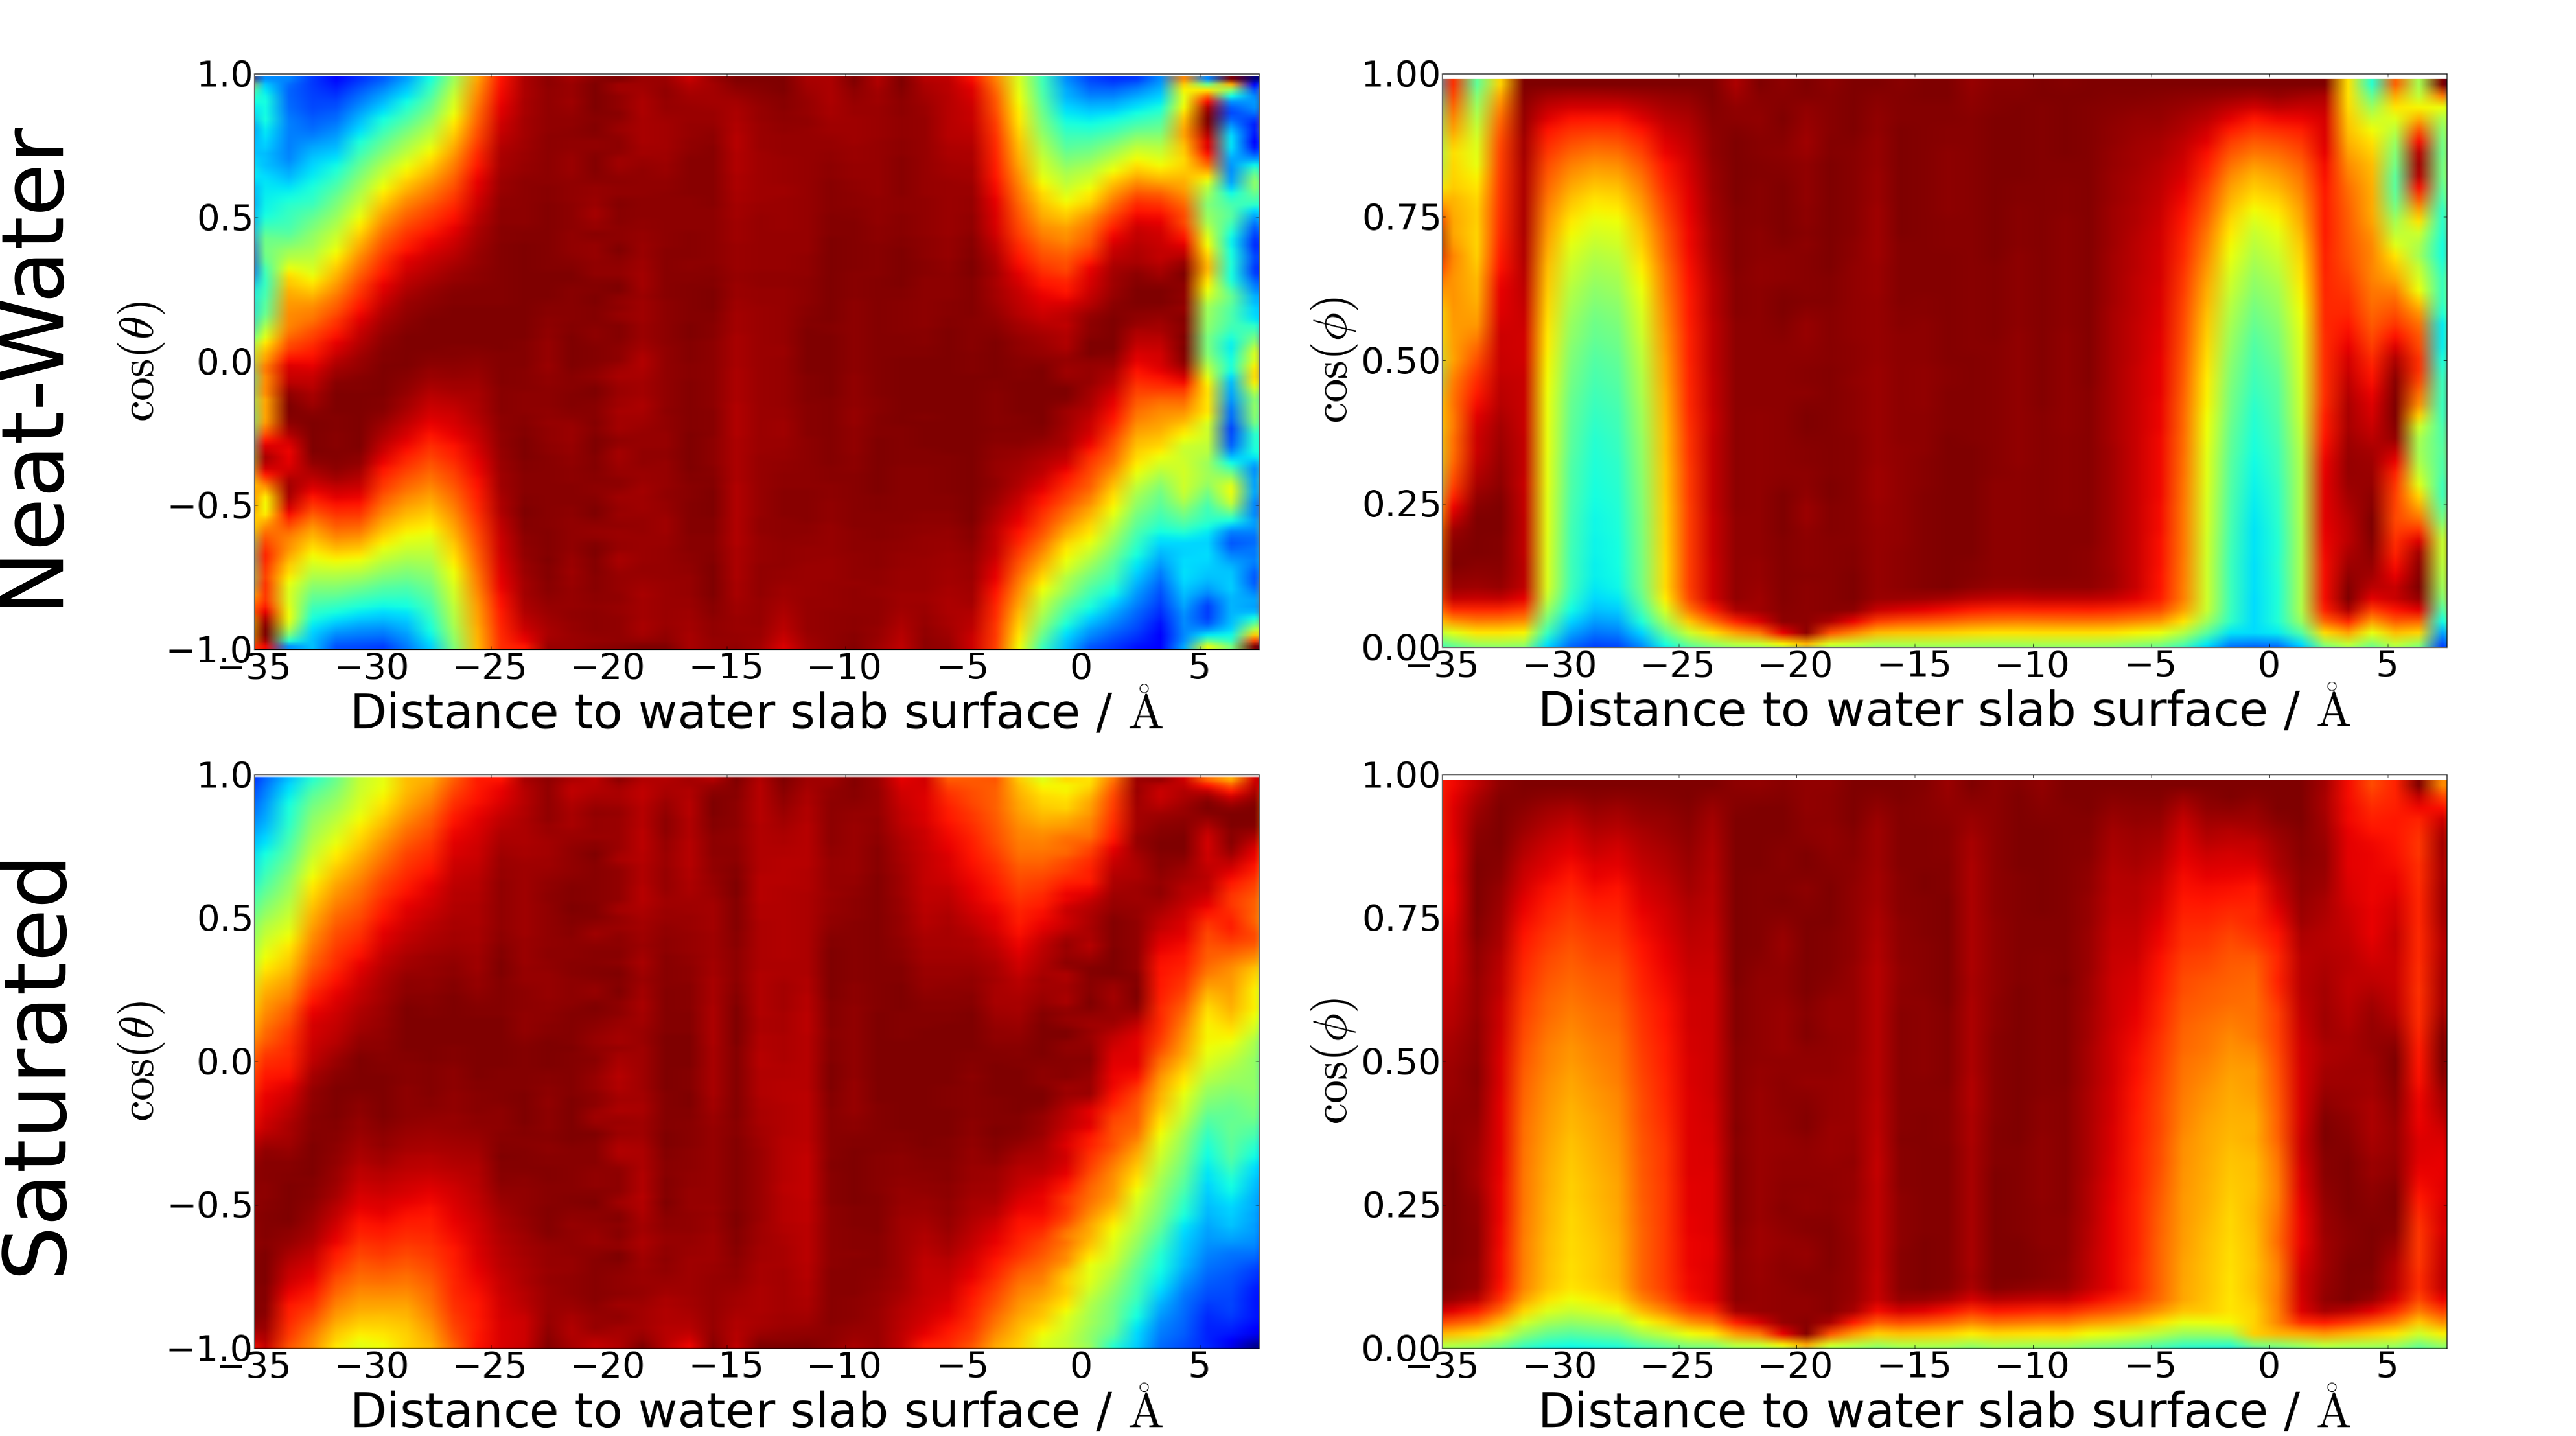
\includegraphics[scale=1.0]{images/h2o-angles/h2oangles.png}
		\caption{Molecular orientation histograms of \wat~throughout the surface equilibrated systems. The top surface is located at a distance of 0 with negative positions in the bulk of the slab. The bottom slab surface is approx. 30\angs~below the top surface. Shown are the angle distributions for $\theta$ (left column) and $\phi$ (right column) in both the neat-\wat~system (top row) and the saturated system (bottom row). The distributions are normalized to account for the changing number of water molecules at different positions in the system.}
		\label{fig:water-orientation}
	\end{center}
\end{figure}


\subsection{\suldiox~Orientation}

Orientation distributions of the adsorbed \suldiox~molecules were created during the equilibrium simulations for both the neat-water and saturated systems. Figure \ref{fig:so2-orientation} shows the distributions of $\cos(\theta)$ and $\cos(\phi)$ (arranged similarly to the water orientation distributions plots in figure \ref{fig:water-orientation}). The \suldiox~orientation data set for the neat-water system is much smaller as only a single \suldiox~molecule was simulated in the bulk. The resulting distribution plots are thus noisier than the corresponding saturated plots, but effective comparisons can still be drawn.

Within 5\angs~of the water surface (the approximate distance from the surface that \suldiox~begins interacting with the outer-most waters) the angular distribution of the single \suldiox~(in the neat-water system) is concentrated primarily in $\cos(\theta)>0$. The peak of the distribution occurs at $\cos(\theta)=1$. The \suldiox~bisector points out of the water surface, with the sulfur atom pointing towards the aqueous bulk, and the two oxygens pointing into the gas phase. This same distribution occurs in the saturated system for positions below 5\angs. Beyond 5\angs~above the surface both distributions become isotropic. Promixity to the water highly orients the \suldiox~with the sulfur atom pointing in towards the water bulk. Moving further away from the water surface, and interacting less with \wat~molcules allows for greater orientational freedom as exhibited in the isotropy of the distributions above 5\angs. %Because both the neat-water and saturated systems show rather similar distributions, it is possible that the concentration of \suldiox~does not strongly affect the orientation of the \suldiox, unlike the orientations of waters.

The plots of $\cos(\phi)$ are both isotropic, although the neat-water system plot is quite noisy from the small data set. Because the \suldiox~near the surface is oriented perpendicularly to the interface, the $\cos(\phi)$ orientation is expected to be isotropic. Further from the water surface where the bisector orientation becomes isotropic, the $\cos(\phi)$ distribution also becomes isotropic. For the \suldiox~orientation, the $\phi$ angle does not provide further information regarding the surface behavior.

\begin{figure}[h!]
	\begin{center}
		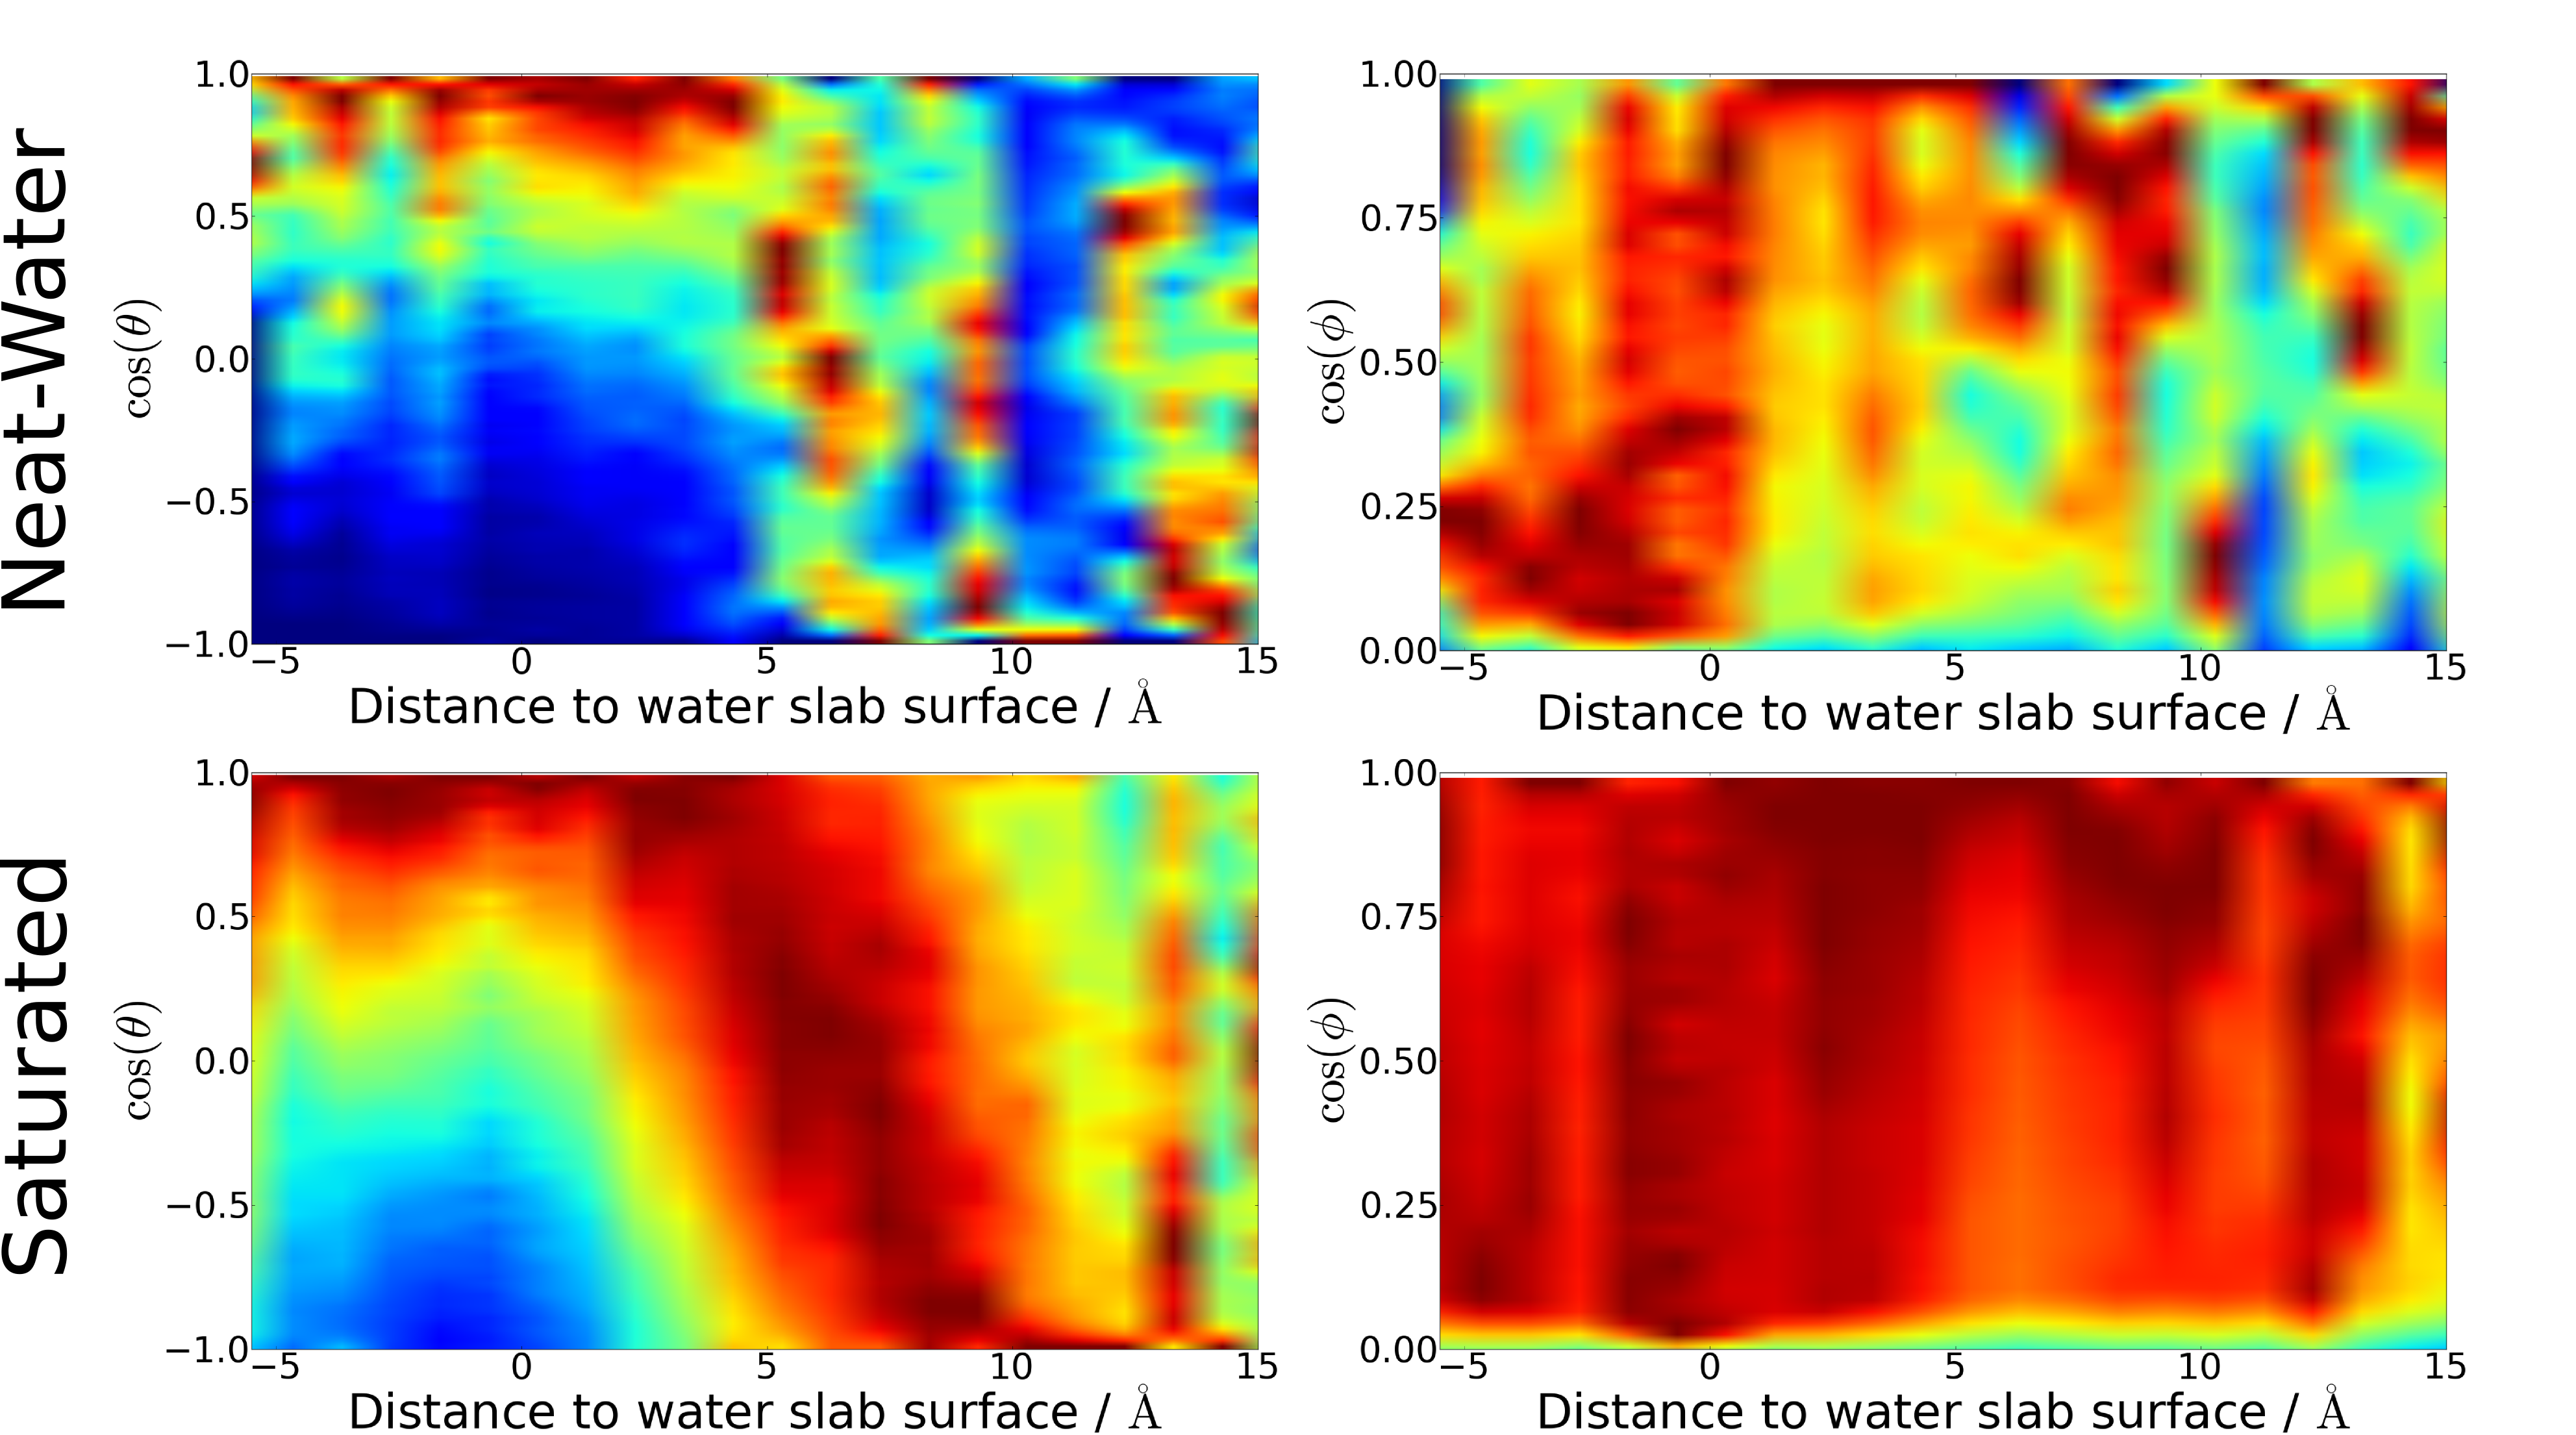
\includegraphics[scale=1.0]{images/so2-angles/so2-angles.png}
		\caption{Molecular orientation distributions for \suldiox~molecules adsorbed to the water slab surface. Distributions are shown for $\cos(\theta)$ (left column) and $\cos(\phi)$ (right column) for both the neat-water (top) and saturated (bottom) systems. For both systems the $\theta$ distributions show \suldiox~bound to the water surface with the sulfur pointing towards the water slab, and the oxygens pointing to the gas phase. In this configuration the $\phi$ distribution is isotropic because of the water slab's in-plane symmetry.}
		\label{fig:so2-orientation}
	\end{center}
\end{figure}
